\documentclass[a4paper, 11pt]{article}
\usepackage{comment}
\usepackage{amsmath}
\usepackage{mathtools}
\usepackage{algorithm}
\usepackage[noend]{algpseudocode}
\usepackage{fullpage}
\usepackage{graphicx}
\graphicspath{ {images/} }
\begin{document}
\title{Final Project Report (CSE 519): Ranking arXiv papers}
%\subtitle{(Appointment time: 2nd slot on 11th December at 4 PM)}
\date{\parbox{\linewidth}{\centering%
  \today\endgraf\bigskip [Appointment time: 2\textsuperscript{nd} slot on 11\textsuperscript{th} December at 4 PM]}}
  
\author{Amol Damare \\ adamare@cs.stonybrook.edu \\SBU ID: 107914028
\and
Punit Mehta \\  pmmehta@cs.stonybrook.edu \\SBU ID: 111461860}
\maketitle

\section{Introduction}
In this project, we consider a problem of ranking an arXiv paper. Specifically, we try to rate/rank a paper in a network consisting of other relevant papers based on how popular the paper is. Ranking a scientific paper is a non-trivial task even for a field expert. We tried to solve some aspect of such paper ranking by transforming the underlying problem to predict a `score' of a node in a graph. In particular, we create a citation graph from our dataset and apply deep-walk to generate the latent representations of each paper. Later, we consider different machine learning models to rank the papers in the citation graph based on such representations in our training data. 

\vspace{0.5cm}

The organization of the report is as follows: In section 2, we start with the motivations on how we model our problem using latent representations. In section 3, we describe our general approach that we use across all the models to rank a paper. In section 4, we comment on our naive baseline model and some of its limitations. Section 5 proposes a better baseline model based on our leanings from the observations on the previous baseline. We outline an advanced model in Section 6 that we extensively evaluate in Section 7 and 8 comparing it with the two proposed baselines using various evaluation techniques. We show some results of our advanced model in Section 9 and conclude the report in Section 10.

\section{Social behavior of scientific papers}
A paper can be related to another paper through various ways such as - one paper cites other paper, both papers cite the same paper, they are accepted in the same journal/conference, they can have the same authors etc. We can use these relationships to form a network or graph of papers. When we think of scoring these papers, we can say that score of a paper will be dependent on the scores of the papers it is connected to in such graph. There is a correlation between scores of connected papers. So, when we have a new paper we can score it by looking at the scores of the papers it is connected to. In this way, network of papers behaves similar to any social network. This relationship allows us to apply recent developments in social relational learning \cite{deepwalk}  ,\cite{tang2011leveraging}to our problem. Also it allows us to model our problem as a relational learning problem \cite{tang2009scalable}, \cite{tang2009relational}. 

\section{Our approach}
The basic approach that will be used in scoring papers is given in Algorithm \ref{alg:algo1}
\begin{algorithm}
\caption{High level algorithm to get ranks of papers}
\label{alg:algo1}
\begin{algorithmic}[1]
\State Create a graph of papers capturing relations such as citations, authors, conferences etc.
\State Get latent social embeddings for the vertices of this graph. 
\State Create train and test data using some helper ranking function.
\State Train a model on this embedding to predict the score/rank of paper.
\end{algorithmic}
\end{algorithm}
Now, we will go in details of each step of this algorithm. Step 1 is trivial for our baseline model. We have created the graph using just citations as a criteria to get a citation graph of of papers. It's possible to extend this graph to include other relationships as well, as we have the necessary data to build such graph. Figure \ref{fig:datamodel} shows the fields of our dataset we have for all the papers.


\begin{figure}[h]
    \centering
    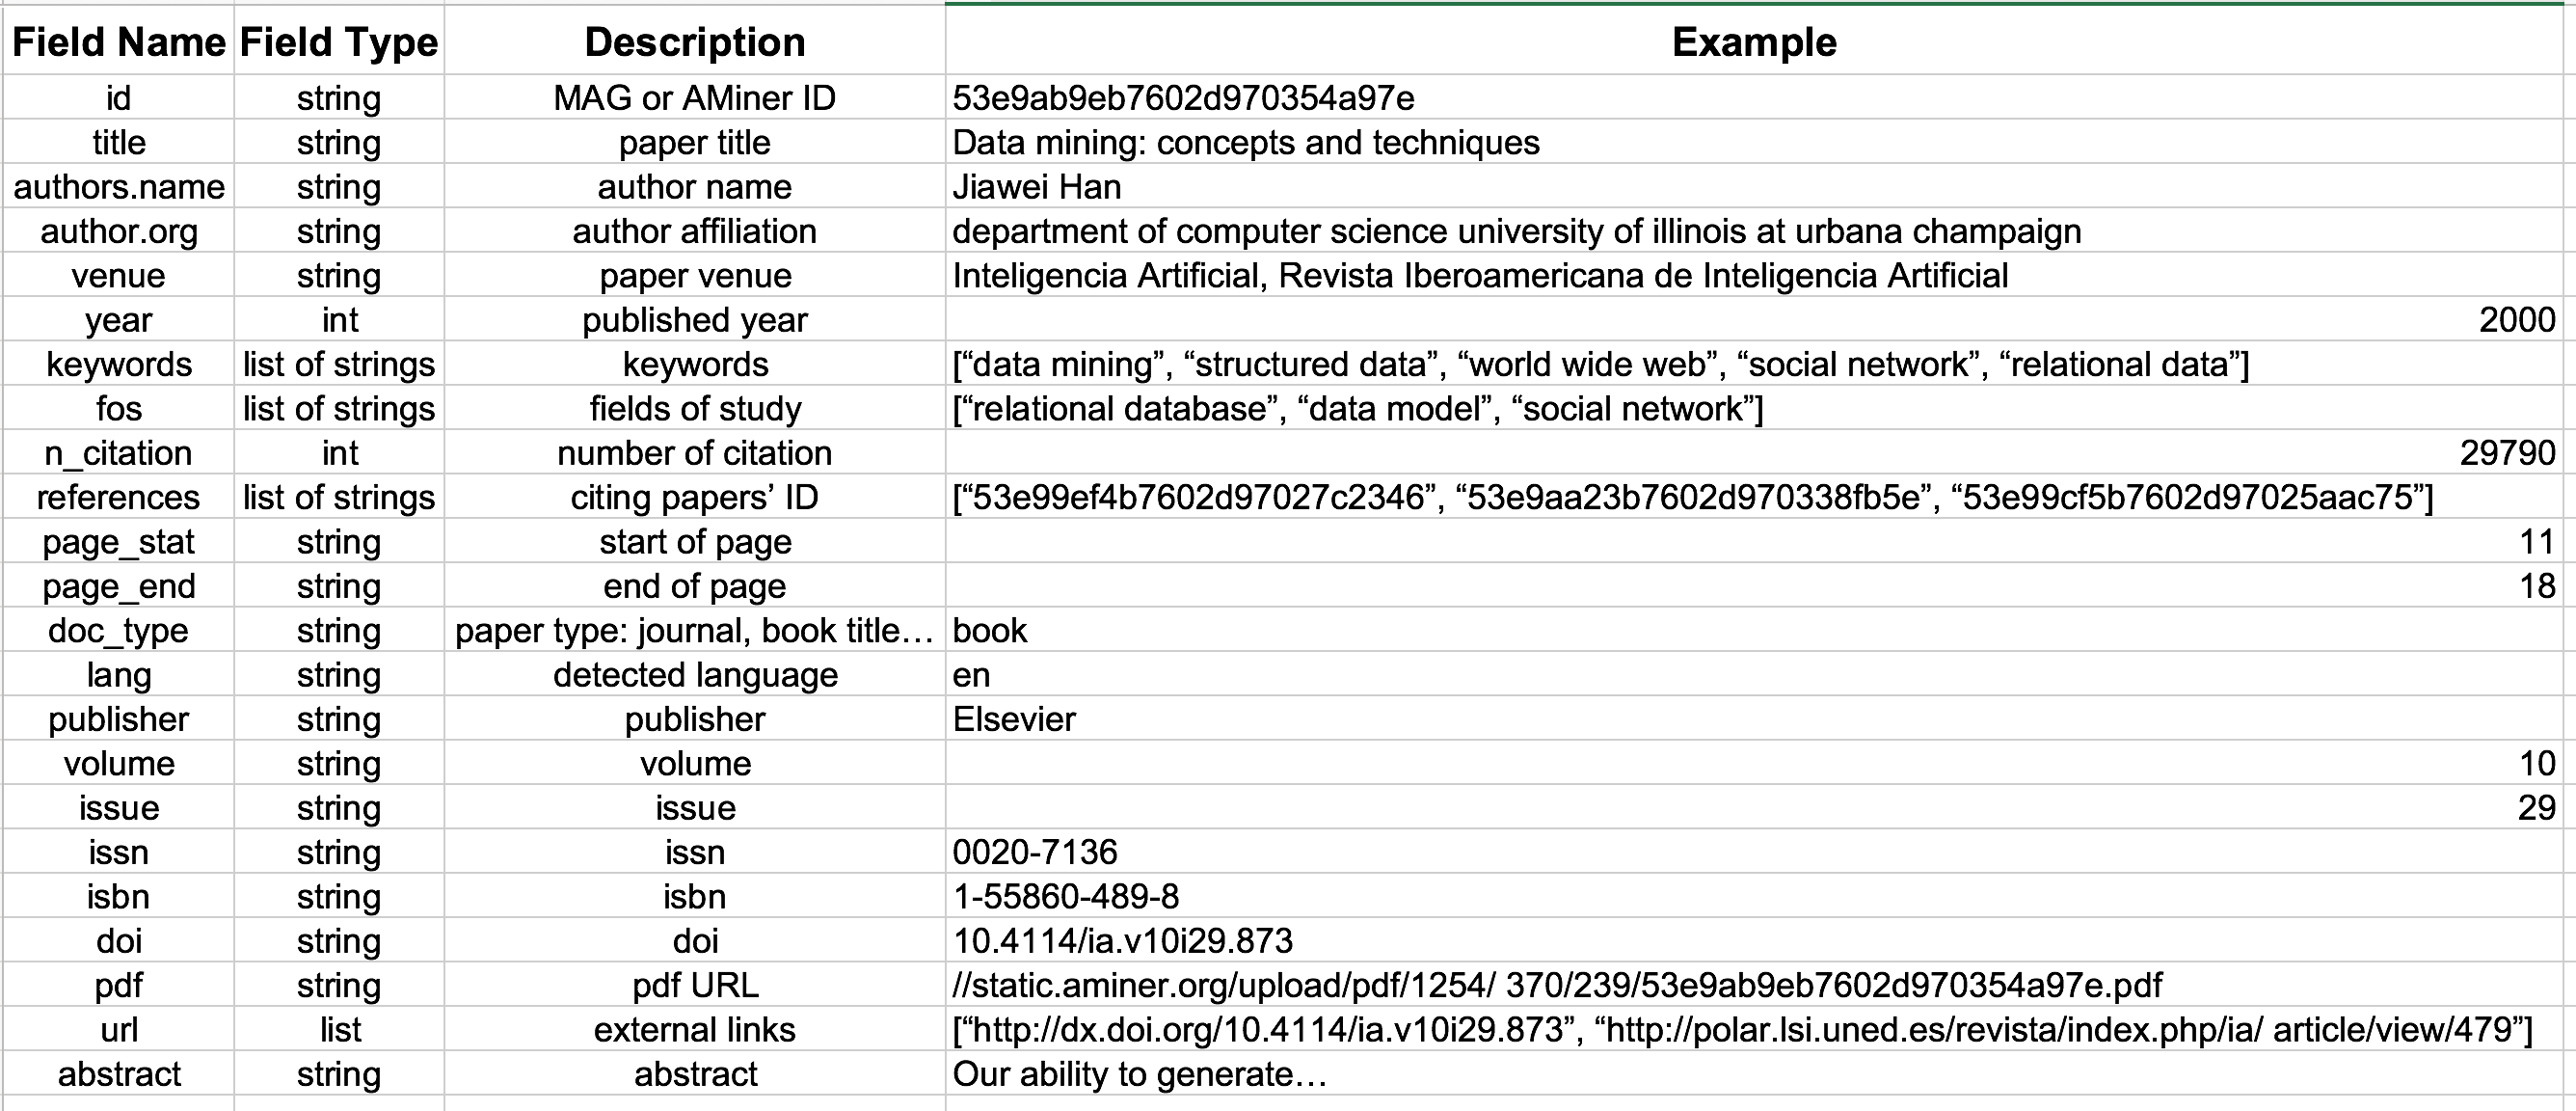
\includegraphics[width=17cm,height=8cm]{datamodel_new}
    \caption{Paper data model and its fields \cite{data}}
    \label{fig:datamodel}
\end{figure}


\subsection{Latent social representation of graph}
In step 2 of our algorithm \ref{alg:algo1}, we need to get latent social representation of the graph we constructed in step 1. We have used `DeepWalk' algorithm presented in \cite{deepwalk} to get the social embedding of the citation graph. DeepWalk applies deep learning techniques to learn the latent social representations of each vertex in the network. To do this \cite{deepwalk} has presented idea that random walks in graph is similar to short sentences in a special language whose vocabulary is the set of vertices of the network. Hence, we can apply same deep learning techniques that are used in neural language models to learn latent representation of each vertex. We will be using the same algorithm to get the representation of each vertex in our citation graph. There are other methods to get social representation of a vertex such as Spectral clustering\cite{tang2011leveraging} which uses spectral graph theory(eigen values of Laplcian of graph), \cite{tang2009relational} uses eigen values of Modularity matrix of graph etc. Deepwalk works well on all types graph and works very well even if the graph is sparsely labeled in relational classification task \cite{deepwalk}, which is exactly kind of representation we would need to rank the papers as we have very huge graph (166,192,182 vertices) often with very sparse labeling (as we will be using experts to rank few papers). 

\subsection{Intuitive Ranking Helper Function}
We don't have any intuitive way to rank or score papers based on social representations we got from running DeepWalk on the graph. Also, it is very difficult to get a generalized scoring/ranking function that works universally well. But if we just consider one of the parameters to decide if a paper is good or not then we can have an intuitive ranking function that we can easily explain. But this ranking function does not generalize well. In this project, we propose the idea that we generalize this naive but intuitive ranking function by training some regression model on latent social representation of the graph. 

\section{Baseline (1) : Venue score is equivalent to a paper score}
\subsection{Idea}
Initially, we considered a naive function that ranks a paper based on the conference or journal it was accepted in. (We can easily get the impact factors of conferences and journals and we follow the intuition that if a venue at which the paper is published is good then paper is as good as the venue itself.) Using this naive intuitive function to score a paper, we trained a linear regression model with input vectors as deep-walk's latent representations (using semi-supervised learning). In this baseline model, graph was constructed using citations and our ranking helper function was only considering conferences that these papers were published in. Algorithm \ref{alg:algo2} and  \ref{alg:algo3} give detailed dynamics of the model. The detailed evaluation on this model is presented in Evaluation section.

%\subsection{Prediction of the score/rank of a paper} 
%To rank/score the papers, our initial approach was to get the feature vectors from deepwalk and then come up with a function of this feature vector to get the score of the paper. But after getting these feature vectors for each paper we came to conclusion that its very hard to interpret what each of this dimension represent intuitively. e.g. does feature 0 represent citation relation or does it represent author relation etc.  So it was hard to come up with a function which would make sense and give us good results for all the papers. We have a powerful tool in our hand in the form these feature vectors we got from deepwalk, and we want to utilize their full potential. So we tried to model ranking as a regression problem. Let's say we have ranks/scores of some of the papers then we can easily train a model on feature vectors to predict the rank or score of the rest of the papers. And as show in deepwalk paper such model works well even in very sparsely labeled dataset such as youtube \cite{deepwalk}.  So for our baseline model we ranked few papers manually.  We have used the ranks of conferences or journals to get estimate of rank/score of paper that was published in that particular conference/journal. We have made an assumption that if conference/journal is good then paper accepted in that journal/conference will be a good paper too. We used this logic to create the training dataset for our models.

\begin{algorithm}
\caption{Algorithm for Baseline model (1)}
\label{alg:algo2}
\begin{algorithmic}[1]
\State Create graph $G(V,E)$ using citations.
\State $G_{train}, G_{test}$=Split($G$) \Comment{Get random papers from graph to create training and testing datasets}
\State IntuitiveRankingHelperFunction($V_{train}$)
\State IntuitiveRankingHelperFunction($V_{test}$)
\State Initialize F as array of feature vectors
\State F=DeepWalk(G) \Comment{This runs deepwalk on graph to get vector representation of each vertex }
\State $model$=LinearModel($G_{train},F$)\Comment{Initialize a linear model}
\State Evaluate  $model$ on $G_{test}$
\State ranks=model.predict(G)
\State return ranks
\end{algorithmic}
\end{algorithm}
\begin{algorithm}
\caption{Algorithm for intuitively ranking papers}
\label{alg:algo3}
\begin{algorithmic}[1]
\Procedure{IntuitiveRankingHelperFunction}{$V$}
\State Initialize VenueRank table \Comment{this table has ranks of each conference and/or journal}
\For {$v in V$}
	\State $rank[v]=rank[Venue[v]]$ \Comment{Naive way to rank the paper, Paper is as good as conference/journal it is published in}
\EndFor
\State return $rank$
\EndProcedure
\end{algorithmic}
\end{algorithm}

\subsection{Observations}

During the experiments with this baseline model, as the prediction of linear regression model highly depends on the output features in the training data (paper scores which in fact are venue scores for our model), we found that it's really important to give an appropriate score to each paper if we want to predict a reasonable score. 

\vspace{0.2cm}


When we tested our baseline model (1), we found that some lower values in the rating-scale were missing due to the missing conferences in our training dataset as our intuitive ranking function completely depends on the venue-score. Hence, we need a better way to rank the papers in the first place in order to predict them better later.

%This is desirable property for our model as we want the model to generalize and take in to consideration other affiliations of the paper as well while scoring. $R^2$ value of our model is $0.095534$, which is indicates that our model not that good and can be improved. Figure \ref{} shows the p-test result for our model. Our p-value is. 0.043, which indicates that our model is good and we can reject the null hypothesis.  \\
%\\From the evaluation of our model it is clear that hypothesis we made are actually true. We can say that approach we are using works and we can make further progress by improving our model to get good results. We also shown that "DeepWalk" indeed captures the relationship which are not explicit at the time of creation of graph. We created the graph using citations and still got good results when we trained the model to basically predict the relationship based on conferences. 

%\begin{table}[h!]
%\centering
%\begin{tabular}{||c c c ||} 
% \hline
% Data Set & Training &  Testing \\ [0.5ex] 
% \hline\hline
% Mean Error &  1 & 13.97\% \\ [1ex] 
%Median Error & 1  & 13.87\% \\ [1ex] 
% \hline
%\end{tabular}
%\caption{Error rates for linear regression base model}
%\label{table:1}
%\end{table}
%\begin{figure}[h]
%    \centering
%    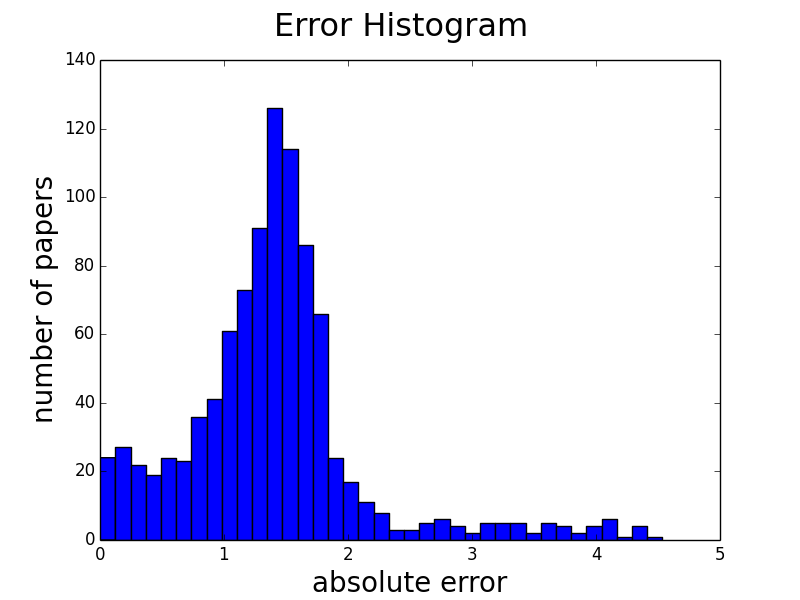
\includegraphics[width=17cm,height=8cm]{figure_1}
%    \caption{Error histogram of baseline model}
%    \label{fig:errorhistogram}
%\end{figure}
%\begin{figure}[h]
%    \centering
%    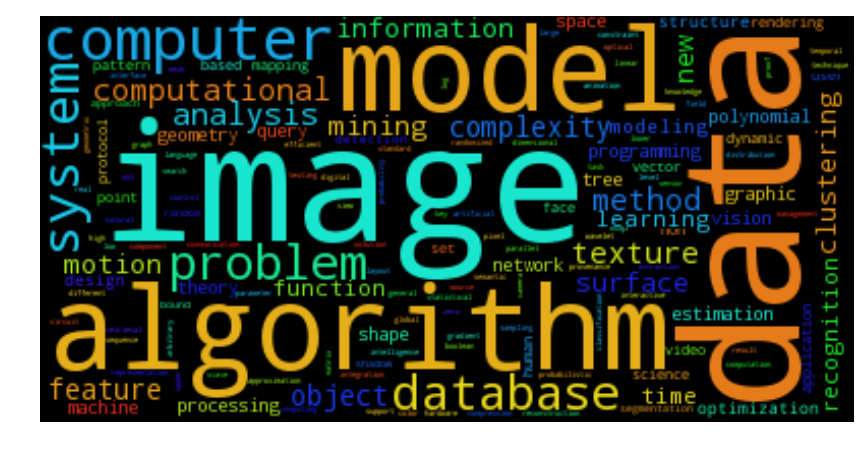
\includegraphics[width=16cm,height=7cm]{venue-image}
%    \caption{Most prominent topics in computer science}
%    \label{fig:venue}
%\end{figure}
%\begin{figure}[h]
%    \centering
%    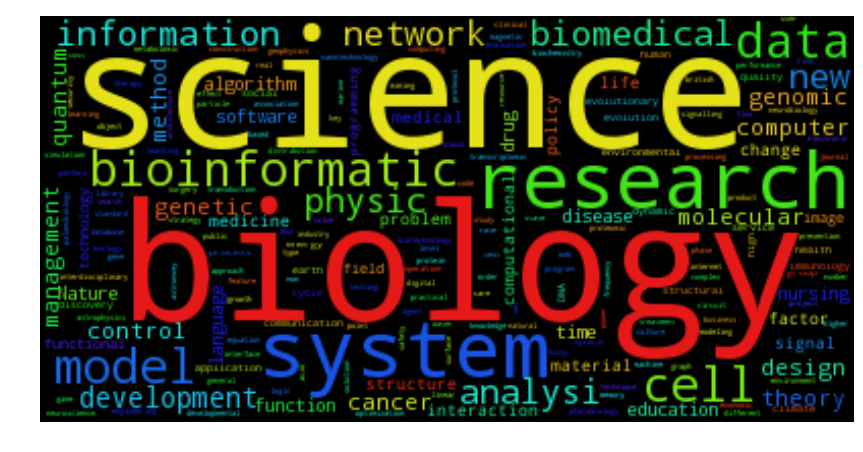
\includegraphics[width=16cm,height=7cm]{visual-gen}
%    \caption{Most prominent general topics}
%    \label{fig:topic}
%\end{figure}
%\begin{figure}[h]
%    \centering
%    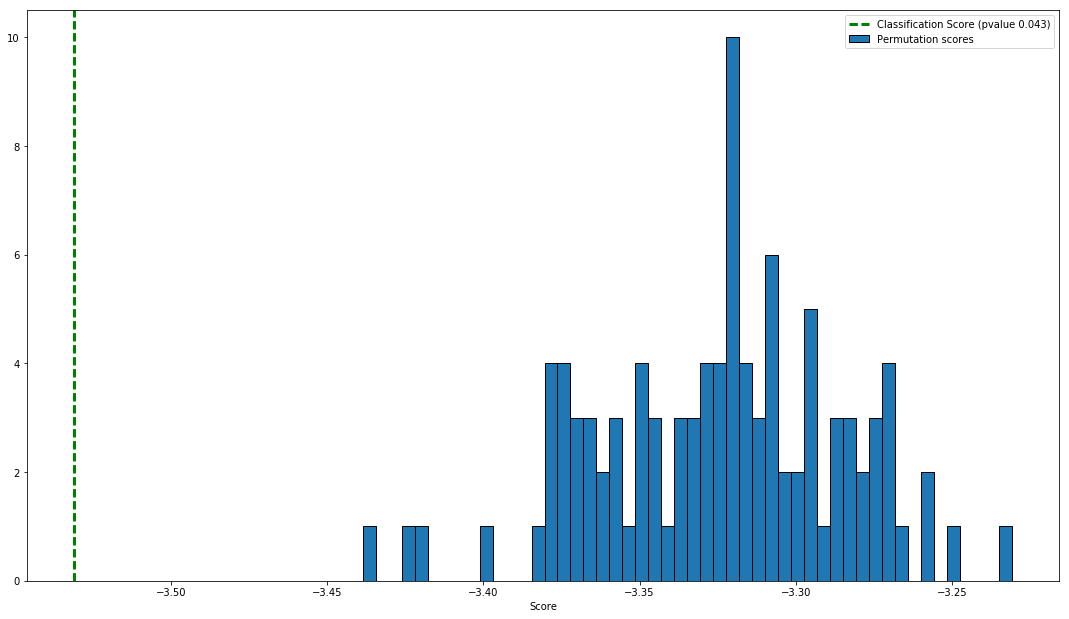
\includegraphics[width=16cm,height=9cm]{permutation_test}
%    \caption{P-test for model}
%    \label{fig:ptest}
%\end{figure}

\begin{figure}[!htb]
    \centering
    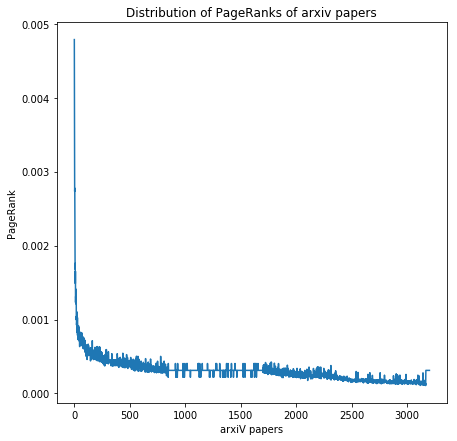
\includegraphics[width=7cm,height=7cm]{pagerank-distribution}
    \caption{PageRank Ratings}
    \label{fig:pagerank-distribution}
\end{figure}

\section{Baseline (2) : PageRank as a scoring function}

\subsection{Idea}
As we noted in the previous section, our baseline model (deep-walk on citation graph and linear regression on the deep-walk's parameters) highly depends on the score that we initially give to each paper (semi-supervised learning). If we can't give a reasonable rating to the papers in the first place, the linear regression will be trained on mostly erroneous data and the output prediction might not be helpful. Hence, to improve our base-line model, we clearly focus on the ways we can attach a score to a paper in order to create a trainable dataset. One of the most popular choices of giving a rank to a graph of nodes is PageRank \cite{pagerank}.

\vspace{0.5cm}

Therefore, we again create a citation graph of all the papers and run PageRank algorithm on the ciration graph as part of our new baseline model. This way, we get a rank of each paper in the dataset and we can treat it as a score of our training dataset. The output of the PageRank algorithm is shown in Figure \ref{fig:pagerank-distribution}. Note the power law distribution generated by PageRank here. Here, x-axis corresponds to various arXiv papers and y-axis is rating generated by PageRank.

\subsection{Linear regression using PageRank score}

Now, we have a citation graph with scores from page rank algorithm and we generate the deep-walk representations for the same. The feature vector of deep-walk has 64 dimensions (which is a smaller representation of a node in such a huge citation graph) and is an input feature to our Linear Regression model. Here, we believe that since deep-walk representations capture the social relations between the nodes in the citation-graph, it's a good idea to train on them as academic papers connected to (referred by or being referred in) a paper with good score likely to be a good paper. 

\vspace{0.5cm}

We train the regression model on latent representations of deep-walk (our input feature) and the scores (our output value) we got from PageRank algorithm. The trained model should predict the score of a paper given the latent representation of it in the citation graph. We evaluated this model on the previous baseline model and other competitive models. We noticed a significant improvement in the residual graph of this new baseline model. Detailed results are explained in the Evaluation section.

\section{Advanced model : PageRank + DeepWalk + kNN}
\subsection{Idea}
Intuitively, we believe that similar nodes (based on the out-degree of a node) in the citation-graph should be given similar scores. We note that we construct the graph in such a way that out-degree of a node corresponds to the number of citations of a paper mapped to that node in the network. To exploit such similarities, it's a good idea to apply k Nearest Neighbors algorithm to the DeepWalk feature vectors as DeepWalk also in some sense captures the same notion in a social graph.

\vspace{0.5cm}

Hence, we start with rating the papers using PageRank (similar to what we did for our improved baseline model) and generate DeepWalk representations. We take these feature-vectors (number of dimension = 64) along with the PageRank scores and apply k Nearest Neighbors algorithm in order to train our mode. We use a different subset of our dataset than the one used to train the model in order to test this advanced model so that we can see how well our advanced model generalizes. The evaluation on the test dataset is presented in the Evaluation section with more details. Here, the optimal value of k is 4 that we got by trying out various possibilities and observing the results. In the next section, we detail out the evaluation strategy and compare the results we got for all three models.

\section{Evaluation}

We consider five methods to evaluate all of our three models and compare them with each other: (1) Residual graphs of the error in prediction, (2) Citations of a paper as an evaluation metric, (3) Confusion Matrix of our ratings, (4) Error Histogram, (5)  General error-scores (mean square, training/testing error etc.) We end the evaluation section by showing the permutation-test results of our advanced model.

\subsection{Residual graphs of error in prediction}

For Residual graphs, we plot the error in prediction (i.e prediction score - actual score) and see how the error points are distributed for each predicted value. We can see a trend of improvement from \ref{fig:residual_first_baseline} to \ref{fig:residual_knn} as the points are tending towards a random distribution from linear around the zero-error.

\vspace{0.5cm}

For our Baseline Model (1), we don't get the score which is less than 6. This is surprising as testing dataset is a random sample of our entire dataset and should ideally follow the same distribution that we have in our training dataset. We debugged down the issue and found that since we manually give scores to the conference, there are some conferences for which we don't have papers in our testing dataset and hence, linear regression couldn't predict the smaller values corresponding to the papers published in those less prestigious journals. Hence, we missed the lower values. That infact was one of our motivations to apply PageRank to all the papers and have an unbiased score that solely depends on the structure of the citation graph.

\vspace{0.5cm}

For our Baseline Model (2), we can see a linear trend around zero error and our kNN model has an almost random distribution in that region. Hence, we conclude that kNN performs better than our previous two baselines. 
 
\begin{figure}[!htb]
\minipage{0.32\textwidth}
  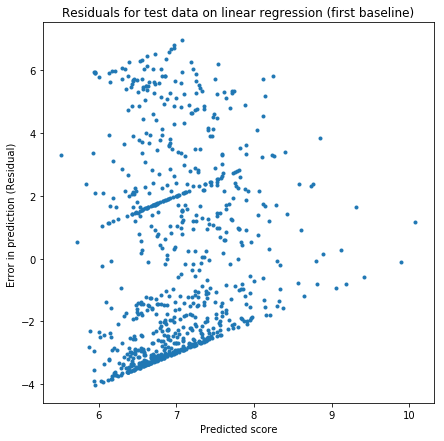
\includegraphics[width=\linewidth]{residual_first_baseline.png}
     \caption{Residual plot: Baseline (1)}
    \label{fig:residual_first_baseline}
\endminipage\hfill
\minipage{0.32\textwidth}
    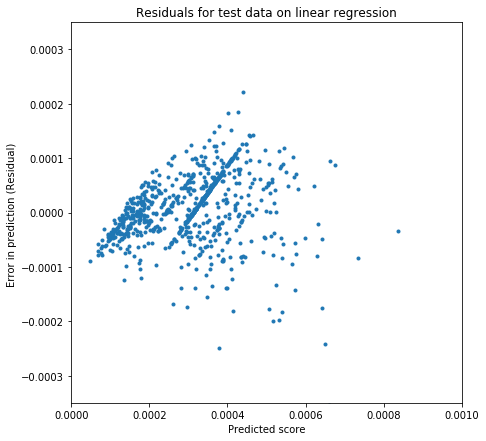
\includegraphics[width=\linewidth]{residual_second_baseline.png}
    \caption{Residual plot: Baseline (2)}
    \label{fig:residual_second_baseline}
\endminipage\hfill
\minipage{0.32\textwidth}%
  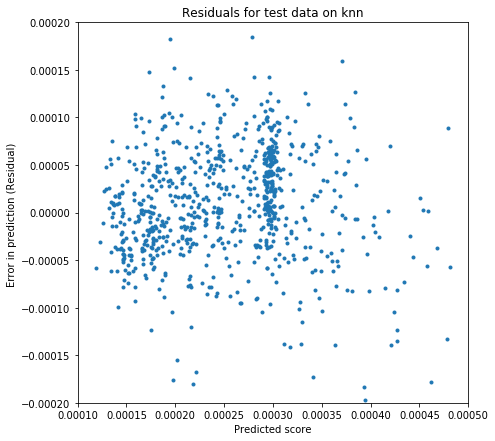
\includegraphics[width=\linewidth]{residual_knn.png}
    \caption{Residual plot: kNN}
  \label{fig:residual_knn}
\endminipage
\end{figure}




%
%\begin{figure}[h]
%    \centering
%    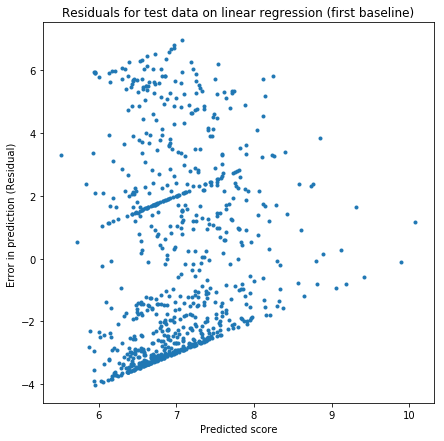
\includegraphics[width=7cm,height=7cm]{residual_first_baseline}
%    \caption{Residual plot - Baseline model (1)}
%    \label{fig:residual_first_baseline}
%\end{figure}
%
%\begin{figure}[h]
%    \centering
%    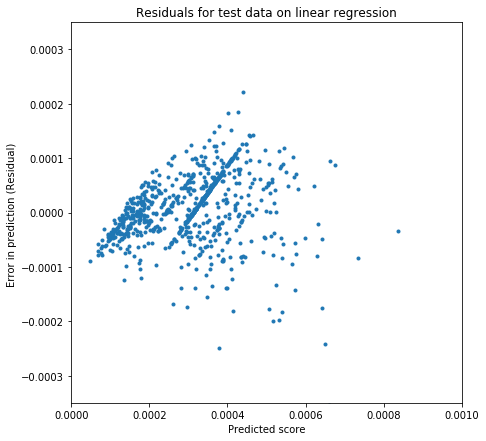
\includegraphics[width=7cm,height=7cm]{residual_second_baseline}
%    \caption{Residual plot - Baseline model (2)}
%    \label{fig:residual_second_baseline}
%\end{figure}


\subsection{Citations as an evaluation metric}

The second evaluation technique that we consider is about inferring the correctness of prediction from the citations of a paper. The fact that papers with high citations should relatively have higher score helps us in determining how well our models are scoring as against the citations of papers. For such an evaluation we plot the Figures \ref{fig:citation_rank_lr_old}, \ref{fig:citation_rank_lr} and \ref{fig:citation_rank_knn}. We split the citations in three windows colored red, green and black (that is red points correspond to papers with citations from 0 to 3, green from 4 to 10 and black from 10 to higher values)

\vspace{0.5cm}

As we can see that, our baseline model (1) gives higher scores to papers with very low citations (red points on the right) and some papers with high citations are given relatively low score (green points on the left). This behavior is less observed in baseline model (2) and kNN tries to cluster the papers with similar number of citations. In that regard, kNN works better here. However, it does have some outliers (black points on the left with very low score) and kind of under-performs for such papers.

\begin{figure}[!htb] 
\minipage{0.32\textwidth}
  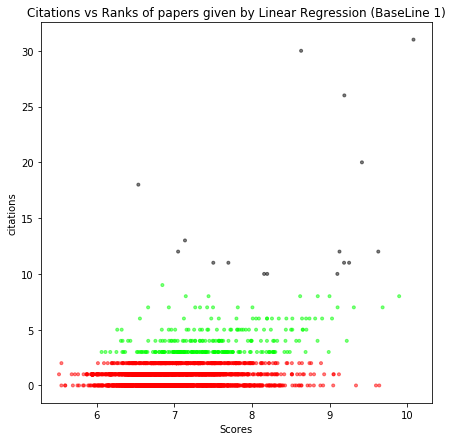
\includegraphics[width=\linewidth]{citation_rank_lr_old.png}
     \caption{citations vs rating: Baseline (1)}
    \label{fig:citation_rank_lr_old}
\endminipage\hfill
\minipage{0.32\textwidth}
    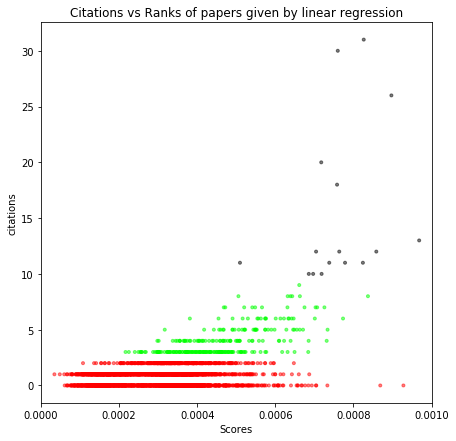
\includegraphics[width=\linewidth]{citation_rank_lr.png}
    \caption{citations vs rating: Baseline (2)}
    \label{fig:citation_rank_lr}
\endminipage\hfill
\minipage{0.32\textwidth}%
  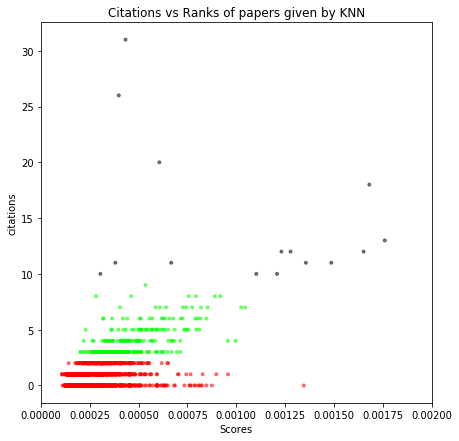
\includegraphics[width=\linewidth]{citation_rank_knn.png}
    \caption{citations vs rating: kNN}
  \label{fig:citation_rank_knn}
\endminipage
\end{figure}


\subsection{Confusion matrix}
We have confusion matrix for our three models that we considered in this project as shown in Figures \ref{fig:confmat_lr}, \ref{fig:confmat_lr_2} and \ref{fig:confmat_knn}.  We divided the scores we got from pagerank and scores we got from our model into 10 different bins to get the true and predicted label for each paper.
\vspace{0.5cm}

For baseline model (1), we can again observe that it doesn't predict any values which is less than 6 irrespective of what the actual score of the paper is. However, papers corresponding to lower actual values (true label) are given relatively low score (that is 6,7 in predicted label) and we can see papers with high predicted label when we approach high values in actual score. Having observed that, we can see a significant scope of improvement in this model. Baseline model (2) performs better than model (1) to distribute the papers across entire matrix in a meaningful way. However, we can still see many papers which are misclassified here as there are small values in the diagonal of its confusion matrix. The confusion matrix for kNN looks acceptable as there are high values in the diagonal and almost all the diagonal values are filled up and can conclude that kNN does a pretty good job here in rating the papers.

\begin{figure}[!htb] 
\minipage{0.49\textwidth}
  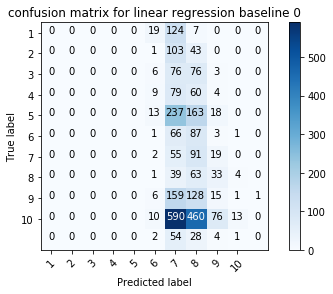
\includegraphics[width=\linewidth]{confmat_lr.png}
     \caption{Confusion Matrix: Baseline (1)}
    \label{fig:confmat_lr}
\endminipage\hfill
\minipage{0.49\textwidth}
    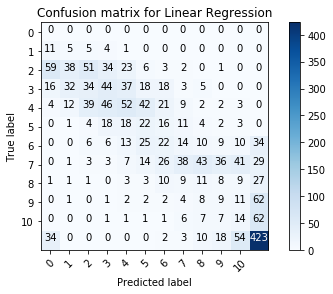
\includegraphics[width=\linewidth]{confmat_linear_new.png}
    \caption{Confusion Matrix: Baseline (2)}
    \label{fig:confmat_lr_2}
\endminipage\hfill
\end{figure}

\vspace{0.5cm}

\begin{figure}[!htb] 
\minipage{0.49\textwidth}%
  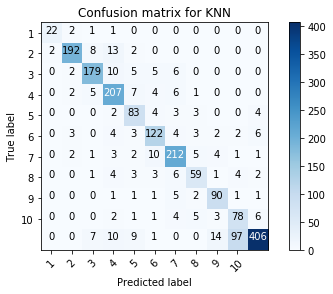
\includegraphics[width=\linewidth]{confmat_knn_new.png}
    \caption{Confusion Matrix: kNN}
  \label{fig:confmat_knn}
\endminipage\hfill
\minipage{0.49\textwidth}%
  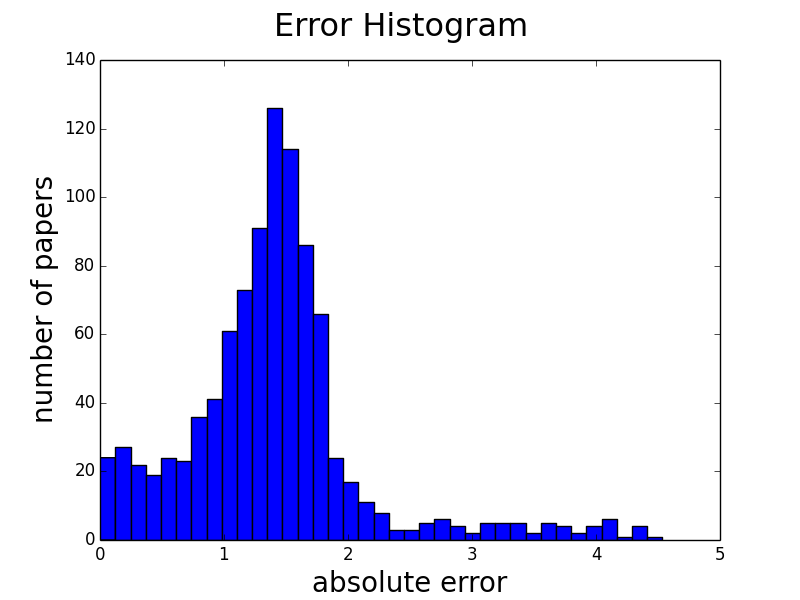
\includegraphics[width=\linewidth]{error_hist_linear_old.png}
   \caption{Error Histogram: Baseline (1)}
  \label{fig:error_hist_linear_old}
\endminipage\hfill
\end{figure}

\subsection{Error histograms}

We plot error histograms for both the baseline models and kNN as show in Figures \ref{fig:error_hist_linear_old}, \ref{fig:error_hist_linear} and \ref{fig:error_hist_knn}. We notice a reasonably good error-histogram for kNN and  can see that most of the errors are completely centered around zero.

\begin{figure}[!htb] 
\minipage{0.49\textwidth}%
  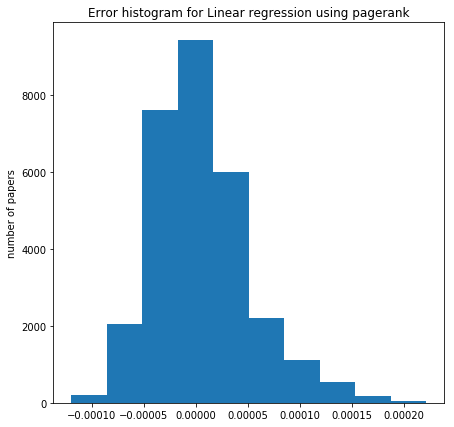
\includegraphics[width=\linewidth]{error_hist_linear.png}
   \caption{Error Histogram: Baseline (2)}
     \label{fig:error_hist_linear}
\endminipage\hfill
\minipage{0.49\textwidth}%
  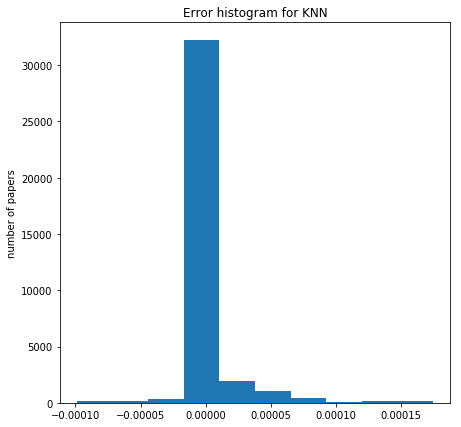
\includegraphics[width=\linewidth]{error_hist_knn.png}
   \caption{Error Histogram: kNN}
  \label{fig:error_hist_knn}
\endminipage\hfill
\end{figure}

\subsection{General error-scores}

We have tabulated the important error values for our new baseline and kNN in Figure \ref{fig:error_table}. We can see a decline in the error values for our kNN model from our baseline model.

\begin{figure}[!htb] 
\minipage{0.49\textwidth}%
  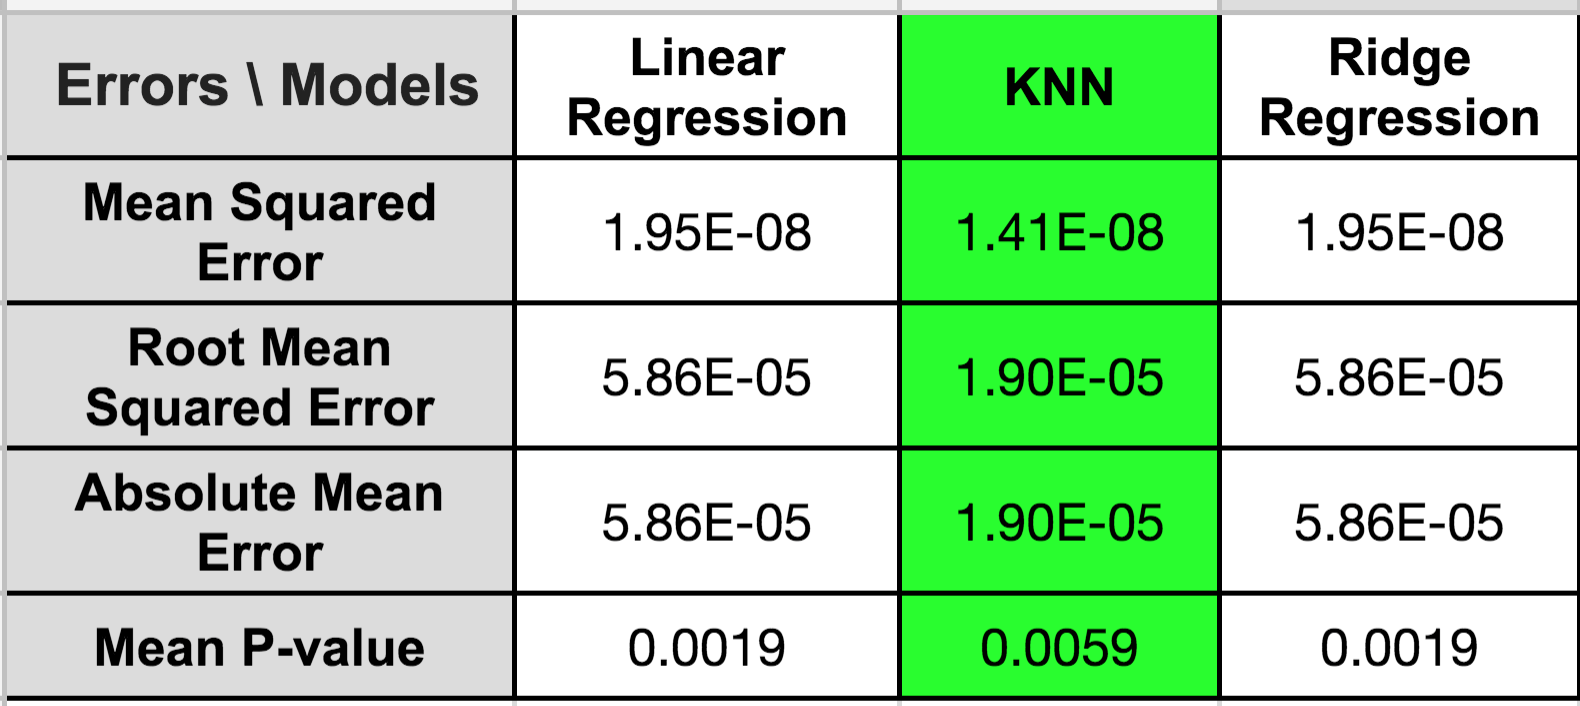
\includegraphics[width=\linewidth]{error_table.png}
   \caption{General error values}
     \label{fig:error_table}
\endminipage\hfill
\minipage{0.49\textwidth}%
  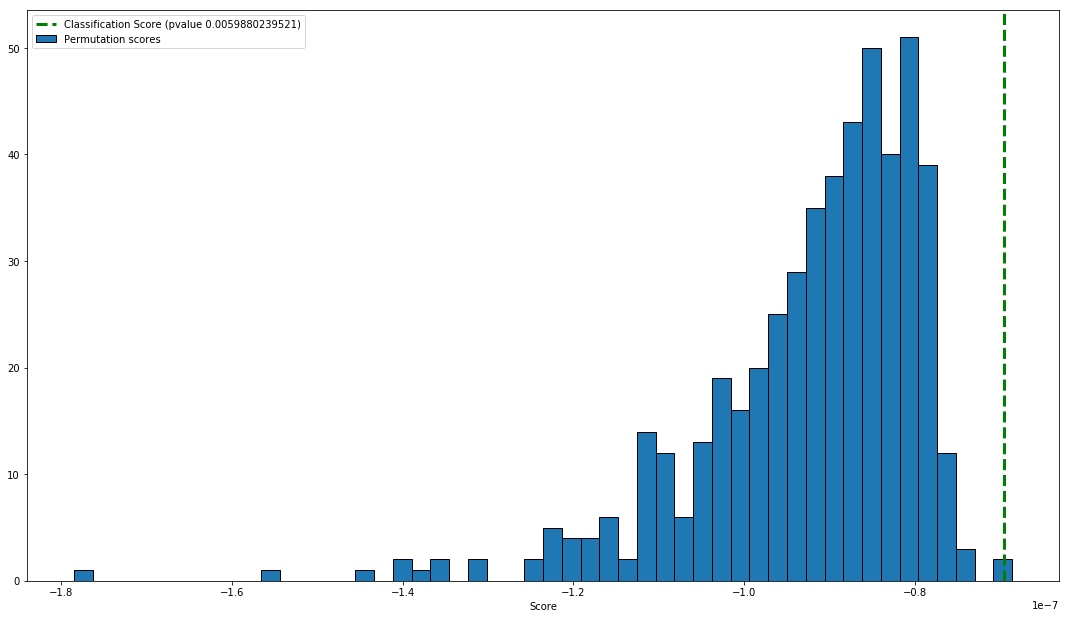
\includegraphics[width=\linewidth]{ptest_knn.png}
   \caption{Permutation Test: kNN}
  \label{fig:ptest_knn}
\endminipage\hfill
\end{figure}

\subsection{P-test on advanced model}

We performed a p-test on our advanced model that uses PageRank, DeepWalk and kNN and the results are shown in Figure \ref{fig:ptest_knn}. Our p-value is 0.005 for kNN.  The p-test just proves that our models are better than just predicting on random noise. We have already shown in our evaluation using confusion matrix and residual graphs that kNN works much better.
\section{Ridge Regression}

During our analysis, we observed that the residual graph of linear regression (Figure \ref{fig:residual_first_baseline}) has some linear trend and were trying to understand it. That time, we found that if we have such linear trend, ridge regression is a good model to try for prediction. However, we got almost the same results (shown in Figures \ref{fig:residual_ridge_regression}, \ref{fig:error_hist_ridge}, \ref{fig:confmat_ridge}) as we got for linear regression and didn't notice any substantial difference.

\begin{figure}[!htb] 
\minipage{0.32\textwidth}
  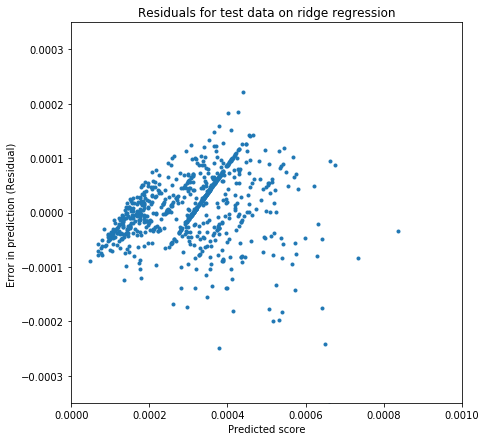
\includegraphics[width=\linewidth]{residual_ridge_regression.png}
    \caption{Residual Graph: Ridge Regression}
  \label{fig:residual_ridge_regression}
\endminipage\hfill
\minipage{0.32\textwidth}
    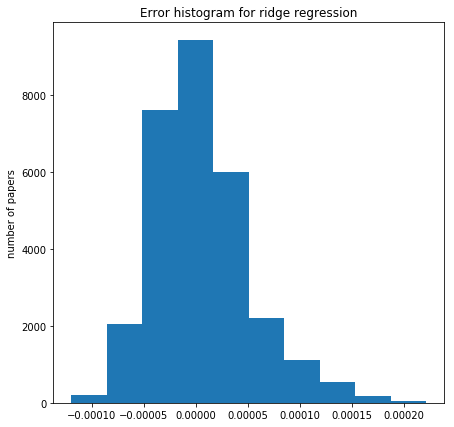
\includegraphics[width=\linewidth]{error_hist_ridge.png}
    \caption{Error Histogram: Ridge regression}
    \label{fig:error_hist_ridge}
\endminipage\hfill
\minipage{0.32\textwidth}%
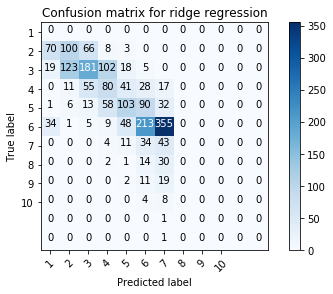
\includegraphics[width=\linewidth]{confmat_ridge.png}
     \caption{Confusion Matrix: Ridge Regression}
    \label{fig:confmat_ridge}
\endminipage
\end{figure}


\section{Results of Advanced model}
In this section, we show the results of our advanced model that we apply to our dataset. We basically listed out two types of papers: Top-5 and Bottom-5. Figure \ref{fig:top_five} and \ref{fig:bottom_five} show the respective category of papers from our dataset.

\begin{figure}[!htb] 
\minipage{0.95\textwidth}%
  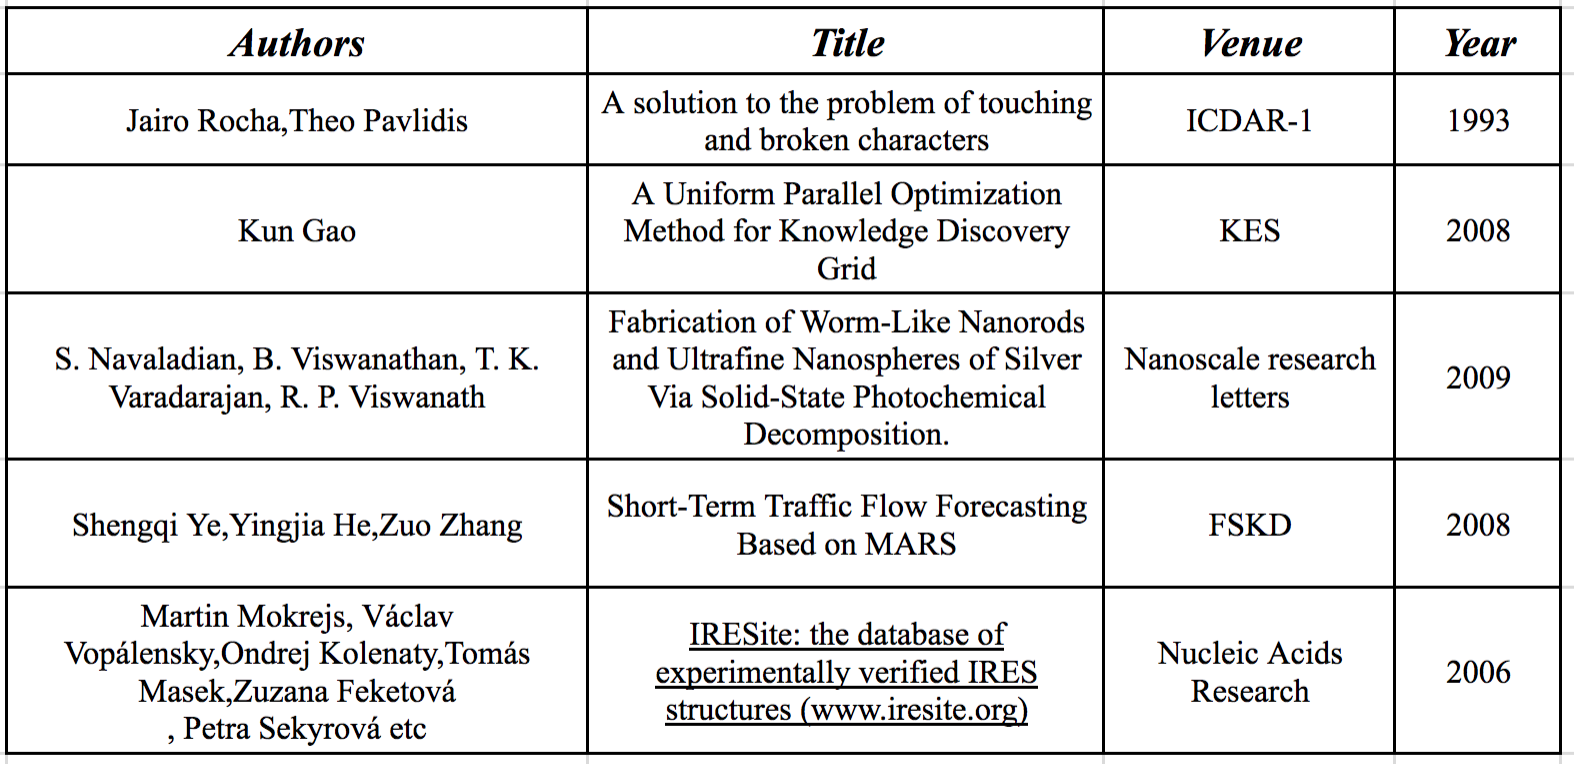
\includegraphics[width=\linewidth]{top_five.png}
   \caption{Top-5 papers}
     \label{fig:top_five}
\endminipage
\end{figure}

\begin{figure}[!htb] 
\minipage{0.95\textwidth}%
  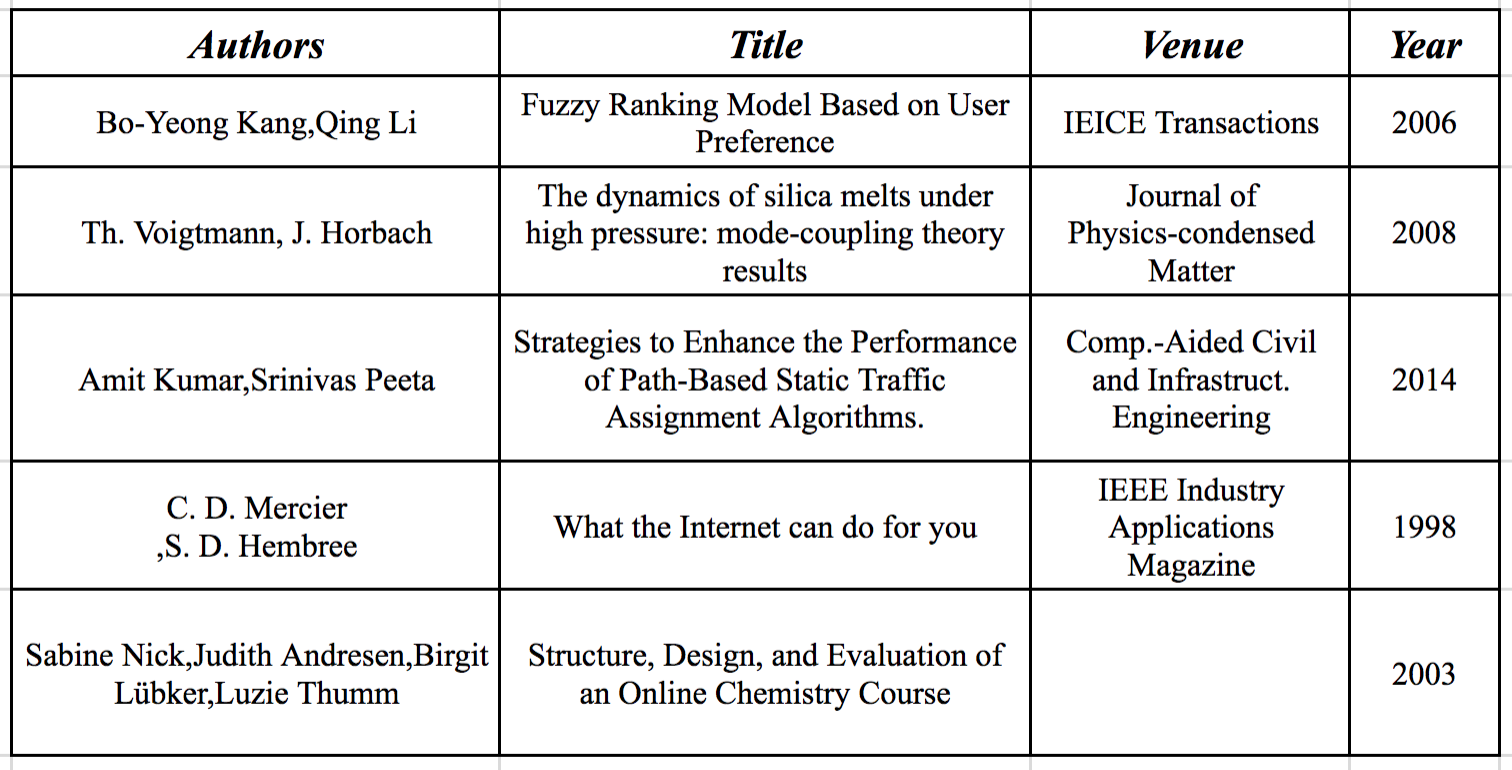
\includegraphics[width=\linewidth]{bottom_five.png}
   \caption{Bottom-5 papers}
  \label{fig:bottom_five}
\endminipage
\end{figure}


\section{Conclusion}

As part of the course project for CSE 519 (Data Science Fundamentals), we tried to rate the academic papers. Specifically, we converted such rating problem to a graph problem (i.e. citation graph) and  rank the nodes of the graph. We devised a naive baseline model to begin with and observed some of its limitations. We improved the baseline by proposing a modified version of it in which our intuitive scoring function uses PageRank than the scores of the venues. We applied DeepWalk in all of our three models and generate latent representations of the nodes in citation graph in order to exploit their social (structural) behavior in the graph. Later, we proposed an advanced model that applies kNN (k=4) using DeepWalk representations. We evaluated our models using standard evaluation techniques and compare their results with eachother. At the end of evaluation, we argue that kNN (our advanced model) performs better than the baselines and does a fair job in rating the papers though it does have some false positives and true negatives.

\section{Code Repository}

We have made our code public. It can be found at https://github.com/amoldamare/CSE519-Project. 

%As seen from results we presented we can see that ranking function really depends on our helper function and the graph we constructed using papers. We can see now a few ways to improve our model
%\begin{enumerate}
%\item Instead of using a helper function we can get an expert to rank or we can rank ourselves, a small number of papers, so we get a more robust initial estimate of ranks of papers. We think this kind of function will generalize better using our approach.
%\item We can construct graph using various other homophily such as authors, conferences etc. We think more relationship we capture in our initial graph, we will get better results for papers which do not all the information such as citations, conferences etc.
%\item We can also improve model by using non-linear regression model in last step of our algorithm.
%\end{enumerate}
%We will try above approaches in an attempt to improve our baseline model.
%We also think, we will better results if we couple the training of DeepWalk and regression linear model together, similar to the deep learning models used in NLP tasks. And if time permits we want to try this approach. This will also require deep understanding of DeepWalk algorithm at coding level.

\begin{thebibliography}{9}
\bibitem{deepwalk}
Perozzi, B. ,Al-Rfou, R.,Skiena, S.
\newblock DeepWalk: Online Learning of Social Representations
\newblock Proceedings of the 20th ACM SIGKDD International Conference on Knowledge Discovery and Data Mining
\newblock KDD '14
\bibitem{tang2009relational}
Tang, Lei and Liu, Huan
\newblock Relational learning via latent social dimensions
\newblock Proceedings of the 15th ACM SIGKDD international conference on Knowledge discovery and data mining,2009



\bibitem{tang2009scalable}
Tang, Lei and Liu, Huan
 \newblock Scalable learning of collective behavior based on sparse social dimensions
  \newblock Proceedings of the 18th ACM conference on Information and knowledge management,2009
\bibitem{Hirsch}
J. E. Hirsch.
\newblock An index to quantify an individual's scientific research output, 2005,
\newblock Proc.Nat.Acad.Sci.46:16569,2005;
\newblock arXiv:physics/0508025.
\newblock DOI: 10.1073/pnas.0507655102.
\bibitem{gindex}
Egghe, L.
\newblock  Theory and practise of the g-index
\newblock Scientometrics (2006) 69: 131.
\newblock https://doi.org/10.1007/s11192-006-0144-7
\bibitem{pagerank}
Page, L., Brin, S., Motwani, R., Winograd, T. 
\newblock  The PageRank citation ranking: Bringing order to the web  
\newblock  (Technical Report). Stanford InfoLab.
\bibitem{garfield}
Garfield, E.
\newblock  Citation analysis as a tool in journal evaluation
\newblock Science,178,471-479.
\bibitem{pinski}
Pinski, G.,  Narin, F. 
\newblock Citation influence for journal aggregates of scientific publications: Theory, with application to the literature of physics
\newblock  Information Processing and Management, 12(5), 297-312
\bibitem{data}
Microsoft Academic Graph 
\newblock https://www.openacademic.ai/oag/
\bibitem{arxiv}
arXiv.org
\newblock  https://arxiv.org/
\bibitem {tang2011leveraging}
  Tang, Lei and Liu, Huan
  \newblock Leveraging social media networks for classification
  \newblock Data Mining and Knowledge Discovery,2011,Springer
 
\end{thebibliography}

\listoffigures
\end{document}